\documentclass[a4paper, 12pt]{article}

\usepackage{graphicx}
\graphicspath{ {../Images/} }
\usepackage[utf8]{inputenc}
\usepackage[T1]{fontenc}
\usepackage{textcomp}
\usepackage{amssymb}
\usepackage{newtxtext} \usepackage{newtxmath}
\usepackage{amsmath, amssymb}
\newtheorem{problem}{Problem}
\newtheorem{example}{Example}
\newtheorem{lemma}{Lemma}
\newtheorem{theorem}{Theorem}
\newtheorem{problem}{Problem}
\newtheorem{example}{Example} \newtheorem{definition}{Definition}
\newtheorem{lemma}{Lemma}
\newtheorem{theorem}{Theorem}


\begin{document}

    

\pagebreak

\section{Clase 1}

\subsection{Info de la materia}

\textit{Mail del profesor.} daniel.penazzi@unc.edu.ar

\textit{Temas a ver.}

\begin{itemize}
    \item Coloreo de grafos 
    \item Flujos en network 
    \item Matchings 
    \item Códigos de correción de errores
    \item P-NP (Complejidad computacional)
    \item Inteligencia artifical
\end{itemize}

La materia tiene tres partes: teórico, práctico y proyecto de programación. Solo
la parte práctica tiene promoción (se explica abajo). El final tiene parte
teórica y parte práctica. La parte teórica es demostrar uno de tres teoremas
dados a priori. La parte práctica tiene ejercicios de demostración o pensamiento
y de resolución de problemas.

La parte práctica se promociona si se aprueban los dos parciales, con cualquer
nota $\geq 4$. De promocionarlo, la parte práctica del final no es necesaria.

El proyecto de programación tiene dos partes. La primera es leer un grafo y
cargar los datos al programa. La segunda es un problema de coloreo de grafos. La
fecha de entrega de la parte uno es en dos o tres semanas a partir de hoy
(13/03). La parte importante es la parte 2.

La biliografía está en el programa 2023.

\subsection{Grafos}

\begin{definition}
    Una grafo es una $2$-upla $G = (V, E)$ con $V$ un conjunto cualquiera (finito) y $E
    \subseteq \left\{ A \subseteq V : |A| = 2 \right\} $
\end{definition}


\small
\begin{quote}

\textbf{Nota.} La restricción de finitud es sólo de esta materia. 

\end{quote}
\normalsize

\begin{center}
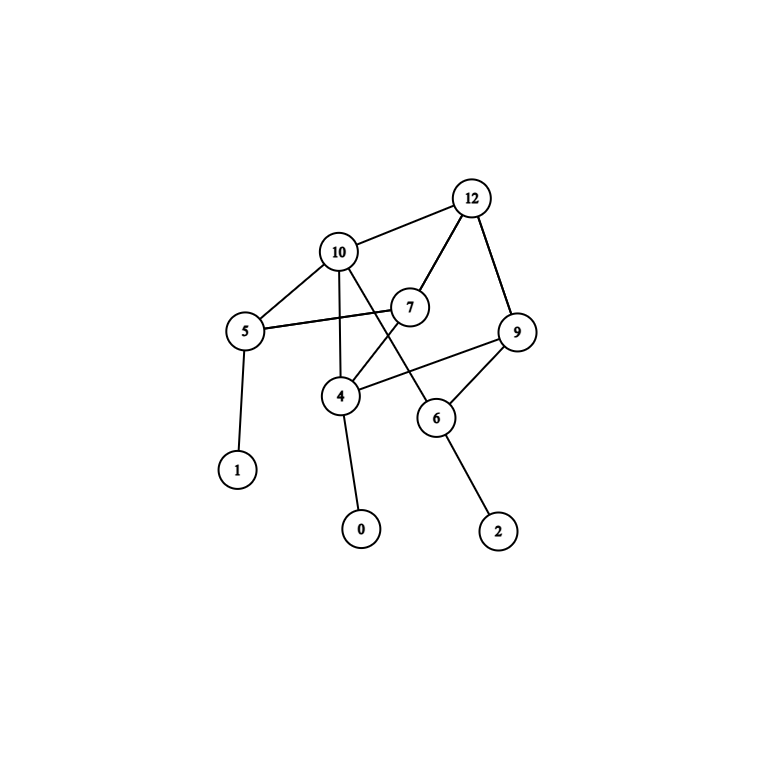
\includegraphics[scale=0.5]{graph}
\end{center}

Los elementos de $V$ se llaman vértices o nodos. Los elementos de $E$ se llaman
lados o aristas. Por convención, a menos que digamos lo contrario, es que $|V| =
n$ y $|E| = m$.

\begin{definition}
    Un camino en un grafo $G = (V, E) $ es una sucesión de vértices $v_1,
    \ldots, v_r$, con $ v_i \in V$ para todo $i$, tal que $\left\{ v_j, v_{j+1}
    \right\} \in E $ para todo $1 \leq j < r$. 
\end{definition}


Dado un camino $v_1, \ldots, v_r$, si $v_1 = x, v_r = y$, decimos que es un
camino de $x$ a $y$. Para todo $G = (V, E)$ definimos la relación binaria 

$$\sim ~:=\left\{ (x, y) \in V^2 : \text{ existe un camino de $x$ a $y$ }  \right\} $$

Es decir, $x \sim y$ denota la relación de que existe un camino entre $x$ e $y$.
Es trivial comproabar que $\sim$ es una relación de equivalencia. Cada clase de
equivalencia $a / \sim$ con $a \in V$ se llama una componente conexa de $G$.

\begin{definition}
    Decimos que $G = (V, E) $ es conexo si y solo si tiene una sola componente
    conexa. Es decir, si $|V / \sim | = 1$.
\end{definition}


\small
\begin{quote}

El profesor no mencionó esto pero es lindo recordar (si alguien ha cursado
lógica) que el conjunto de clases de equivalencia $A / R$ de un conjunto a sobre
una relación binaria $R$ puede en sí mismo darse como un grupo de grafos
disconexos. Por ejemplo, abajo se dan los grafos de un espacio cociente con
siete clases de equivalencia; cada par de vértices unidos por un lado
corresponde a dos elementos equivalentes.


\begin{center}
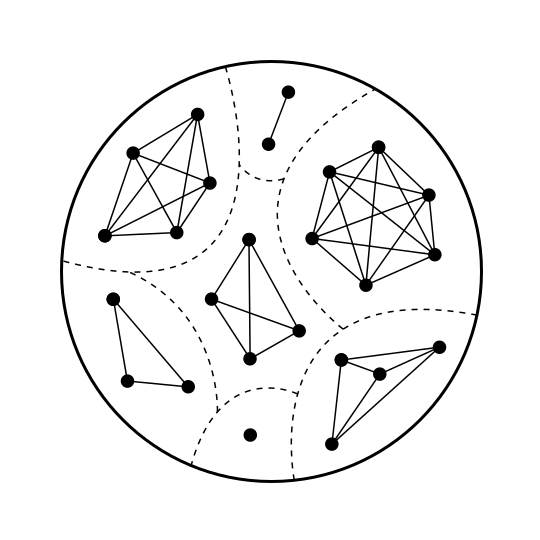
\includegraphics[scale=0.25]{equiv}
\end{center}

Fíjense que de esto se sigue un dato curioso (aunque tal vez irrelevante): Si
$G = (V, E) $ es un grafo conexo con $n$ vértices, el grafo que describe la clase de
equivalencia de $V$ es $K_n$.

\end{quote}
\normalsize

\begin{definition}
    Decimos que un grafo $H = (W, F)$ es un subgrafo de $G =(V, E)$ si
    $W \subseteq V, F \subseteq E$.
\end{definition}

A veces usamos $H \subseteq G$ para decir "$H$ es un subgrafo de $G$", pero no
debe entenderse por esto que $H$ y $G$ son conjuntos.

Observe que no todo $W \subseteq V, F \subseteq E$ satisfacen que $(W, F)$ es un
grafo. Por ejemplo, si $F = \emptyset$ tenemos $F \subseteq E$, pero $F$
no cumple la propiedad de que todos sus elementos sean conjuntos con cardinalidad $2$.

\begin{definition}[Densidad]
    Decimos que un grafo es denso si $m = O(n^2)$. Decimos que un grafo es raro
    si $m = O(n)$.
\end{definition}


\small
\begin{quote}

\textbf{Random fact}. Recuerde que "raro" no sólo significa "inusual" sino que es el
antónimo de "denso". La etimología inglesa es más interesante:
La palabra \textit{Weird} (raro) significaba, en la edad media, destino. Por
eso, en la balada medieval \textit{True Thomas}, se lee "Weird shall never
daunton me": El destino nunca ha de asustarme. Se debe a una antigua leyenda
nórdica en la cual las \textit{Weird sisters}, diosas terribles, tejían el
destino de los hombres. Si le da curiosidad:

https://en.wikipedia.org/wiki/Three_Witches

\end{quote}
\normalsize

\begin{definition}
    Dado $G = (V, E) $, si $x \in V$, $\Gamma(x) := \left\{ y \in V : \left\{ x,
        y\right\}  \in E
\right\} $ se llama el vecindario de $x$. 
\end{definition}

Si $y \in \Gamma(x)$, decimos que $y$
es un vecino de $x$.  El grado de $x$, denotado $d(x)$, es la cantidad de
vecinos de $x$; es decir, $d(x) = |\Gamma(x)|$.
Usamos $\delta = \min \left\{ d(x) : x \in V \right\} $ y $\Delta = \max \left\{
d(x) : x \in V\right\} $. Si $\delta = \Delta$ se dice que $G$ es regular. Por
ejemplo, los
grafos cíclicos y los completos son regulares.

\begin{definition}
    Dado un grafo $G = (V, E) $, decimos que $G$ es regular si $d(x) = d(y)$
    para todo $x, y \in V$.
\end{definition}

Es decir, un grafo es regular si todo vértice tiene la misma cantidad de
vecinos.



\subsection{Repaso de BFS y DFS}

\textit{A completar.}






\subsection{Los grafos $K_n$ y $C_n$}
\label{famosos}

\begin{itemize}
    \item $K_n$ : El grafo completo en $n$ vértices se define 

        $$K_n = \left( \left\{
        1, 2, \ldots, n\right\}, \left\{ \left\{ x, y \right\}  : x, y \in \left\{ 1, 2, \ldots, n
    \right\}  \right\}   \right) $$

    Es el grafo de $n$ elementos donde todos los vértices están conectados unos
    con otros. Resulta que que $m = \binom{n}{2}$. Lo cual implica que $m =
    O(n^2)$.

    \item  $C_n$: El grafo cíclico 

        $$C_n = \left( \left{ 1, 2, \ldots, n \right},
        \left\{ 12, 23, 34, \ldots, (n-1)n, n1 \right\}   \right)$$

        Una observación es
        que $C_3 = K_3$; pero de allí en adelante difieren.
\end{itemize}

\subsection{Coloreo de grafos}

\begin{definition}
    Un coloreo propio de $G = (V, E) $ con $k$ colores es una función  

    \begin{align*}
        C : V \mapsto A
    \end{align*}

    con $|A| = k$ y tal que $xy \in A\Rightarrow C(x) \neq C(y)$.
\end{definition}

Intuitivamente, un coloreo asigna $k$ propiedades a los vértices de modo tal que
ningún par de grafos adyacentes cumple la misma propiedad. 

\small
\begin{quote}

\textbf{Nota.} Hace unos meses escrbí un algoritmo de coloreo en C. Es el
segundo algoritmo dado en esta entrada: 

https://slopezpereyra.github.io/2023-10-29-Hamiltonian/

No prometo que sea muy prolijo o esté bien explicado; ya en general uno es tonto
y encima de tonto no sabe de grafos. Pero tal vez a alguien le sirva, qué se yo.

\end{quote}
\normalsize


\begin{definition}
    El número cromático de un grafo $G= (V, E) $ es 

    \begin{align*}
        \chi(G) = \min_k \left( \exists \text{ coloreo propio de $G$ con $k$
        colores} \right) 
    \end{align*}
\end{definition}

No se conoce un algoritmo polinomial que calcule $\chi(G)$. El proyecto será dar
un algoritmo polinomial que se aproxime a $\chi$.

\subsection{Un algoritmo greedy de coloreo}
~ ~ 

Damos un algoritmo que colorea un grafo $G$ con vértices $v_1, \ldots, v_n$ y
colores $ c_1, c_2, \ldots, c_n  $. Para que el algoritmo
funcione, los colores y los vértices deben tener un orden (en nuestro caso
dado por los subíndices).


\begin{quote}

\textbf{Invariante del algoritmo.} Los coloreos parciales son propios. Es decir,
a medida que se va coloreando iterativamente el grafo, en cada paso el coloreo
resultante debe ser propio.

\textbf{Pasos del algoritmo}. 

\textit{(1)} $C(v_1) = c_1$.

\textit{(2)} $C(v_k) = $ mínimo color que mantenga un coloreo propio (que
satisfaga el invariante).

\end{quote}


\begin{center}
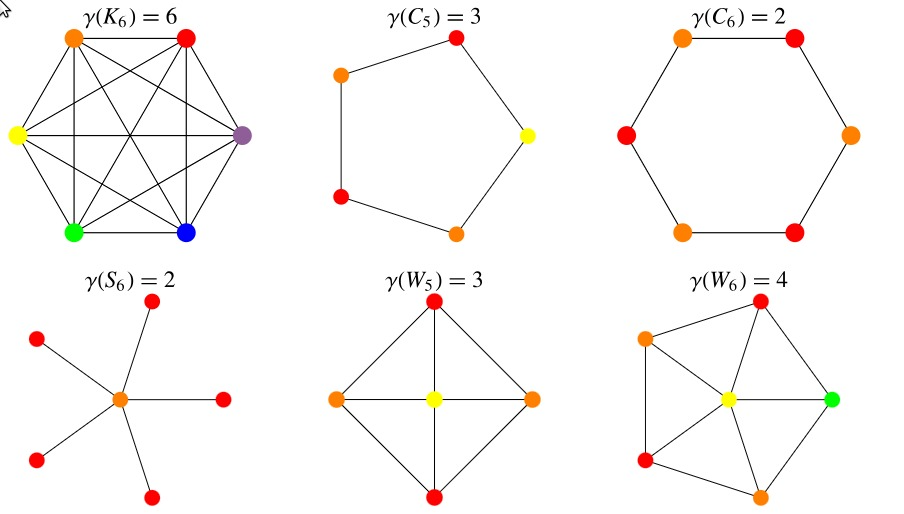
\includegraphics[scale=0.35]{coloring}
\end{center}

\subsection{Acotando $\chi$}

Generalmente nos interesa encontar $\chi(G)$ dado un grafo $G = (V, E) $. Damos
unas pautas y observaciones generales para acotar $\chi(G)$ y así facilitar su
hallazgo.

\begin{lemma}
    Si existe un coloreo propio de $G = (V, E)$ con $k$ colores, entonces
    $\chi(G) \leq k$.
\end{lemma}


\small
\begin{quote}

\textbf{Proof.} Es trivial por definición de $\chi$ ($\chi$ es el mínimo $k$ en
el conjunto de los coloreos posibles de $G$ con $k$ colores).

\end{quote}
\normalsize

El lema significa que para acotar $\chi$ por arriba solo basta dar un coloreo
con $k$ colores.

\begin{lemma}
    Si $H$ es un subgrafo de $G$, $\chi(H) \leq \chi(G)$.
\end{lemma}

Este lema nos dice que podemos acotar $\chi$ por abajo si encontramos un
subgrafo de $G$ cuyo número cromático es conocido. Es fácil ver que $\chi(K_r) =
r$ para todo $r > 1$. Es menos directo pero en clase se demostró que

\begin{align*}
    \chi(C_r) = \begin{cases}
        2 & r \equiv 0 \mod 2  \\ 
        3 & r \equiv 1 \mod 2 
    \end{cases}
\end{align*}

Esto, en combinación con el último lema, nos dice que podemos acotar $\chi(G)$
por abajo simplemente observando si $G$ contiene algún $C_r$  o $K_r$ como
subgrafo. En el caso $C_r$, la cota inferior dada en el caso par, con $\chi(C_r)
= 2$, es trivial (todo grafo necesita al menos dos colores). Por eso nos
quedamos con el siguiente teorema: 

\begin{theorem}
    Sea $G = (V, E) $ un grafo. Si $C_r \subseteq G$ con $r$ impar entonces
    $\chi(G) \geq 3$. Si $K_r \subseteq G$ entonces $\chi(G) \geq r$.
\end{theorem}

\begin{theorem}
    
    Sea $G = (V, E) $ un grafo. Entonces 

    $$\chi(G) = \max \left\{ \chi(C) : C \text{ es componente
conexa de  } G \right\} $$

\end{theorem}


\begin{theorem}
    Sea $G = (V, E) $ un grafo. Entonces $G$ contiene un ciclo impar si y solo
    si $\chi(G) \geq 3$.
\end{theorem}

\small
\begin{quote}

\textbf{Proof.} $(\Rightarrow)$ Trivial. 

$(\Leftarrow)$ Damos una prueba algorítmica. La prueba es simple, pero debe
tenerse presente que usamos \textbf{tres} grafos diferentes en ella: el grafo
$G = (V, E) $ del teorema, una componente conexa $C \subseteq G$, y un grafo
$\mathcal{B} \subseteq C$ resultante de correr BFS de a partir de un vértice de
$C$. El algoritmo determina si $\chi(G) = 2$ y de no serlo construye un ciclo
impar. Usamos la notación $n(z)$ si $z \in V$ para denotar el nivel de $z$ en
$\mathcal{B}$. Dividimos la prueba en tres partes.

\textit{(1)} Como $\chi(G) = \max \left\{ \chi(C) : C \text{ es componente
conexa de  } G \right\} $, tenemos que 

\begin{align*}
    \chi(G) \geq 3 \Rightarrow\exists \text{ c.c. $C$ tal que } \chi(C) \geq 3
\end{align*}

Elegimos $x \in C$ y corremos BFS a partir de él, generando un subgrafo
$\mathcal{B} \subseteq C$ con todos los vértices de $C$ (pero no todos los
lados).

\textit{(2)} Coloreamos cada vértice de $C$ como sigue: como sigue: $c(z)$ será el nivel
BFS de $z$ módulo 2. Esto equivale a hacer $c(x) = 0$ y cada vez que $y$ agrega
a $z$ a la cola de BFS, hacer $c(z) =  1 - c(y)$.

Esto da un coloreo con $2$ colores, pero podría no ser propio (por ejemplo, dos
vecinos de la raíz que son vecinos entre sí tendrían ambos color $1$). Por lo
tanto verificamos si es propio o no. 

\textit{(3)} Si es propio tenemos un coloreo propio de dos colores y $\chi(G) =
2$. Si es impropio, construiremos un ciclo impar. En particular, si no es
propio, existen $u, v \in V$ tales que $c(u) = c(v) $ y $uv \in E$. Pero si
$c(u) = c(v)$, entonces

\begin{align*}
    n(u) \equiv n(v) \mod 2
\end{align*}

Pero en un árbol siempre existe un camino
de la raíz a cualquier vértice arbitrario. Entonces, en $\mathcal{B}$ existe un
camino desde $x$ hasta $u$, y existe un camino desde $x$ hasta $v$. En
particular, existe un vértice $z$ que está en ambos caminos y a partir del cual
los caminos se separan (note que puede ser $x$). Pero en $C$, $uv$ forman un
lado. Luego, en $C$ tenemos el ciclo $z, u, v, z$. 

¿Cuántos lados tiene el ciclo? Vea que de $z$ a $u$ hay $n(u) - n(z)$
lados. De $u$ a $v$ un solo lado, y de $v$ a $z$ otra vez $n(v) - n(z)$.
En total, hay 

\begin{align*}
     n(u) + n(v) - 2 n(z) + 1
\end{align*}

lados. Pero $n(u) \equiv n(v) \mod 2$ y su suma
es par. Luego la suma anterior es impar. Luego existe un ciclo impar en $G$.

\end{quote}
\normalsize

\end{quote}
\normalsize

\begin{theorem}
    Para todo gafo $G = (V, E) $, $\chi(G) \leq \Delta + 1$.
\end{theorem}


\small
\begin{quote}

\textbf{Proof.} Greedy siempre colorea con $\Delta + 1$  colores o menos. Tome
cualquier orden $v_1 \ldots v_n$ sobre $V$. Para colorear $v_i, i \neq 1$, se
mira el color de los vecinos de $v_i$ que son anteriores en el orden.

El peor caso posible es que todos los vecinos sean anteriores en el orden y
todos tengan colores distintos. En ese caso, Greedy descarta $d(v_i)$ colores.
Como $d(v_i) \leq \Delta$, entonces Greedy descarta a lo sumo $\Delta$ colores.
Por lo tanto, siempre habrá al menos un color disponible en $\left\{ 1, 2,
\ldots, \Delta, \Delta + 1 \right\} $.
$\blacksquare$

\end{quote}
\normalsize

Una pregunta natural es si hay grafos cuyo número cromático alcanza la cota
$\Delta + 1$. La respuesta es sí: a saber, 

\begin{itemize}
    \item $\chi(K_n) = n$ y $\Delta = n - 1$.
    \item $\chi(C_{2r+1}) = 3$ y $\Delta = 2$.
\end{itemize}

El siguiente teorema establece que, de todos los grafos conexos, $K_n$ y
$C_{2r+1}$ son los únicos que alcanzan la cota.

\begin{theorem}[Brooks]
    Sea $G = (V, E) $ un grafo conexo distinto de un $K_n$ y un $C_{2r + 1}$.
    Entonces $\chi(G) \leq \Delta$.
\end{theorem}


\small
\begin{quote}

\textbf{Proof.} Complicada, una hora y media o dos de hacer. Triste.

\end{quote}
\normalsize

\begin{theorem}[Baby Brooks o Brooks para bebés]
    Si $G = (V, E) $ un grafo conexo y no regular, entonces $\chi(G) \leq
    \Delta$.
\end{theorem}


\small
\begin{quote}

\textbf{Proof.} Es un caso particular del teorema de Brooks. Corramos BFS$(x)$
con $d(x) = \delta$.
Como $G$ es conexo, obtenemos todos los vértices. Pues los vértices son
agregados iterativamente al árbol del BFS, existe un orden dado precisamente por
el orden de inserción al árbol.

Daremos un orden (que no es el anterior) tal que Greedy colorea $G$ con a lo
sumo $\Delta$ colores. En particular, es el orden inverso al anterior. Es decir
que el último elemento del orden es la raíz $x$.

Como siempre el color del primer elemento es $1$. Sea $z \neq v_1$ (en el orden
del Greedy). El peor caso posible, que $z$ tenga como vecinos a todos los
anteriores, es imposible aquí, porque en el orden de DFS todo $y \neq x$ es
insertado en el árbol por un vértice que ya estaba en el árbol. Y ese vértice
debe ser un vecino. Es decir, en el orden de inserción del BFS, todo vértice
tiene un vecino que es anterior en el orden. Entonces, en el orden inverso, todo
$y \neq x$ tiene al menos un vecino posterior. Entonces, en el peor de los
casos, tiene $d(y) - 1$ vecinos anteriores. Por lo tanto, greedy elimina a lo
sumo $d(y) -
1 \leq \Delta - 1$ colores. $\therefore $ Siempre puede colorear a $y$ con un
color en $\left\{ 1, 2, \ldots, \Delta \right\} $.

Cuando llega a $x$, Greedy elimina a lo sumo $d(x) = \delta$ colores. Y como $G$
no es regular, $\delta < \Delta$. $\therefore $ Existe al menos un color para
$x$ en $\left\{ 1, 2, \ldots, \Delta \right\} $.

\end{quote}
\normalsize


\subsection{¿Para qué acotar $\chi$? Para encontar $\chi$!}

En general no es fácil mostrar que $\chi(G) = \varphi$ de manera directa. Uno
puede mostrar entonces que $\varphi_{l} \leq \chi(G) \leq \varphi_{u}$ usando
las acotaciones vistas antes. Si sucede que $\varphi_l = \varphi_u$ qué bonito
hemos encontrado $\chi(G)$. Si este no es el caso de igual modo estamos
restringiendo el espacio de soluciones posibles. Por ejemplo, si $3 \leq \chi(G)
\leq 4$, tenemos que $\chi(G) = 3$ o $\chi(G) = 4$, y a veces es fácil ver (y
demostrar) cuál de los casos es correcto.

\pagebreak

\subsection{Limitaciones de Greedy}


\textbf{Ejemplo de Greedy mal.} Sea $G = (V, E)$ un grafo tal que $n = 2i$ es par
y 

\begin{align*}
    E = \left\{ xy : x \text{ impar }, y \text{ par }, y \neq x + 1\right\} 
\end{align*}

El grafo es claramente bipartito (un par nunca se conecta con un par, un impar
nunca con un impar) y tiene un coloreo de 2 colores. Sin embargo, al correr
Greedy sobre este grafo, obtenemos un coloreo sub-óptimo.

Se deja al lector verificar los coloreos sub-óptimos que resultan si $n = 2, 4,
6$. Se presenta la siguiente hipótesis inductiva haciendo inducción sobre $i$:


\small
\begin{quote}

\textit{Hipótesis inductiva}. Para todo $j \leq k$, Greedy colorea el grafo con
$c(2j - 1) = c(2j) = j$ colores.

\end{quote}
\normalsize

\small
\begin{quote}

    \textit{Caso inductivo.} Si $j \leq k$ por $HI$ tenemos $c(2j - 1) = c(2j) =
    j$. Si $j = k + 1$, tenemos que $2(k+1) - 1$ es impar y forma lados con
    todos los pares anteriores. Luego greedy no puede asignarle el color de
    ningún par anterior. Es decir, no puede asignar ningún color entre $1$ y
    $k$. Luego greedy lo colorea con $k + 1$. El mismo razonamiento muestra que
    el vértice $2(k+1)$ se colorea con $i + 1$.

    Por lo tanto, greedy colorea $G$ con $\frac{n}{2}$ colores.


\end{quote}
\normalsize


\subsection{Hill clmbing}

Hill climbing es un algoritmo de optimización matemática. Dada una función $f :
\mathbb{R}^n \to \mathbb{R}$ que se quiere maximizar, el algoritmo toma un punto
arbitrario
$\vec{x} \in \mathcal{D}_f$ y evalúa $f(\vec{x})$. Luego se hace $\Delta\vec{x} =
(x_1, \ldots, x_{i} + \epsilon, \ldots, x_n)$ con $\epsilon \in R$ e $i$
arbitario y se vuelve a testear. Si la función incrementa, se hace
$\vec{x} = \Delta\vec{x}$: si no, se hace la modificación inversa. Este proceso
se repite iterativamente hasta que un criterio es satisfecho.

El principal problema del algoritmo de Hill climbing es que encuentra solo
óptimos locales. Para lidiar con este problema, se usa \textit{simulated
annealing}. Si $\Delta \vec{x}$ va mejor se lo acepta; pero si $\Delta \vec{x}$
va peor se otorga una cierta probabilidad de aceptarlo de todos modos. La
probabilidad de aceptar va reduciendo con el tiempo. La idea es permitir la
salida de optimos locales con el tiempo.

En coloreo de grafos, Hill climbing toma la siguiente forma. Se prueba un orden
de $V$ arbitrario y se lo colorea con Greedy. Luego hacer una pequeña
permutación y se prueba de nuevo, etc. 

Existe un modo de asegurarnos que la mutación $\Delta \vec{x}$ de $\vec{x}$
nunca empeore (puede permanecer igual). El problema es que para hacer esto,
reducimos el espacio de búsqueda; es decir, las permutaciones que
exploraremos (las que no pueden empeorar el rendimiento) son muy pocas, y puede
ser que ninguna mejore el rendimiento. 

Una forma de lidiar con esto es elegir varios órdenes iniciales al azar y
aplicar esta idea a cada una de ellas.

\begin{theorem}[VIT]

    Sea $G = (V, E) $ un grafo con un coloreo propio $c$ con $r$ colores $c_1,
    \ldots, c_r$. Sea $V_{c_i} := \left\{ x \in V : c(x) = c_i \right\} $. Sea $P$
    una permutación de $c_1, \ldots, c_r$. Es claro que $P : \left\{ c_1, \ldots, c_r
    \right\} \mapsto \left\{ c_1, \ldots, c_r \right\} $ es una biyección.


    Ordenemos los vértices poniendo primero los vértices de $V_{P(c_1)}$; luego
    los de $V_{P(c_2)}$, etc. Es decir, ordenamos los vértices por bloques de
    color. Entonces Greedy con ese orden usa a lo sumo $r$ colores.
    
\end{theorem}


\small
\begin{quote}

\textbf{Proof.} Hacemos inducción sobre $r$. 

\textit{Caso base $i = 1$.} Los vértices de $V_{P(c_i)}$ tienen el mismo color $P(c_i)$.
Porque $c$ es un coloreo propio, y los vértices en cada $V_{P(c_i)}$ no pueden
formar lados entre sí, Greedy los colorea a todos con el color 1 y usa un color.
$\blacksquare$


$HI(i) \Rightarrow HI(i+1)$: Sea $x \in V_{P(c_1)} \cup  \ldots \cup
V_{P(c_{i+1})}$. Si $x$ está en alguno de los primeros $i$ bloques, Greedy lo
colorea con uno de entre $i$ colores por hipótesis inductiva. 

Si $x \in V_{P(c_{i+1})}$, el
caso en que Greedy lo colorea con un color menor o igual a $i + 1$ no viola lo
que queremos demostrar. Pero asumamos que lo colorea con el color $i +
2$. Entonces ningún color menor estaba disponible; entonces $x$ es vecino de
algún $z$ de color $i + 1$. Pero todos los vértices de $V_{P(c_{i})}$ están
coloreados el color $c_i$. Luego $z \in V_{P(c_{i+1})}$. Pero si
tanto $x, z \in V_{P(c_{i+1})}$ entonces $c(x) = c(z) = P(c_{i+1})$, lo cual
implica que $c$ no es propio. $(\bot)$

\end{quote}
\normalsize

\pagebreak 

\section{Redes y flujos}

Una red es un grafo dirigido con un límite en la información o carga
transferible de un nodo a otro. 

El modelo de problema central es una red de productores y
consumidores. Se trata de encontrar el máximo de información (o producto)
transferible de los productores a los consumidores. Lo transferido de
productores a consumidores se llama flujo. Llamamos a este problema \textit{max
flow}.

\begin{definition}
    Un grafo $G = (V, E) $ con $V$ un conjunto y $E \subseteq V \times V$ se
    llama dirigido.
\end{definition}

Usaremos $\overrightarrow{xy}$ para denotar $(x, y)$ donde $(x, y) \in E$. Observe que
$\overrightarrow{xy} \neq \overrightarrow{yx}$.

\begin{definition}
    Una red o network es una $3$-upla $(V, E, c)$ donde $(V, E)$ es un grafo
    dirigido y $c : E \to \mathbb{R}^{+}$ es una función.
\end{definition}

La función $c$ denota la capacidad de cada uno de los lados.

\begin{definition}[Vecinos]
    Definimos $\Gamma^{+}(x) = \left\{ x \in V : \overrightarrow{xy} \in E \right\} $ y,
    por otro lado,
    $\Gamma^{-}(x) = \left\{ y \in V : \overrightarrow{yx} \in E \right\} $
\end{definition}

Usualmente nos preguntamos no cuánta información puede enviarse de un nodo a
otro, sino cuánta puede enviarse de un conjunto de nodos a otro (de una parte
del grafo a otra). Esto inspira la siguiente notación.

\begin{definition}
    Sea $g : E \to \mathbb{R}$ y sean $A, B \subseteq V$. Definimos  

    \begin{align*}
        g(A, B) = \sum_{x \in A, y \in B \text{ t.q. } \exists \overrightarrow{xy} \in E}
        g(\overrightarrow{xy})
    \end{align*}
\end{definition}

Usualmente usamos la siguiente notación: Si $\zeta$ es una expresión booleana,
$[\zeta]$ es su evaluación en $\left\{ 0, 1 \right\} $. Esto a veces facilita
las cosas; por ejemplo, la definición anterior es equivalente a

\begin{align*}
    g(A, B) = \sum_{\overrightarrow{xy} \in E}[x \in A] [y \in B] [\overrightarrow{xy} \in E] g(\overrightarrow{xy})
\end{align*}

\begin{definition}
    Sea $\mathcal{N} = (V, E, c)$ una network. Sea $x \in V$ y $g : E \to
    \mathbb{R}$. Definimos 

    \begin{align*}
        \text{out}_{g}(x) \sum_{E} [y \in V][\overrightarrow{xy} \in E]g(x) &= g \left(
        \left\{ x \right\}, V  \right) 
    \end{align*}

    Análogamente, 

    \begin{align*}
        \text{in}_g(x) = \sum[y \in V] [\overrightarrow{yx} \in E]g(\overrightarrow{yx}) = g\left( V,
        \left\{ x \right\} \right) 
    \end{align*}
\end{definition}

\begin{definition}
    Dada $\mathcal{N} = (V, E, c)$ una network y $s, t \in V$, una función $f
    :E \to \mathbb{R}$ es un flujo si y solo si 

    \begin{quote}
        
    \begin{enumerate}
        \item $0 \leq f(\overrightarrow{xy}) \leq c(\overrightarrow{xy}) ~ \forall \overrightarrow{xy} \in E$
            (feasability)
        \item $\text{in}_f(x) = \text{out}_f(x) ~ \forall x \in V - \left\{ s, t
            \right\} $ (conservación) 
        \item $\text{out}_f(s) \geq \text{in}_f(s)$ ($s$ es una source o
            productor)
        \item $\text{in}_f(t) \geq \text{out}_f(t)$ (t es un consumidor o sink)
    \end{enumerate}
    \end{quote}

\end{definition}

A veces se pide que lo que entra a $s$ sea cero y lo que salga de $t$ sea cero,
pero esto no es necesario. A fines prácticos, en los ejemplos que veremos esta
última restricción se cumple. Más aún, suele suceder que $\Gamma^{+}(t) =
\emptyset$ y $\Gamma^{-}(s) =\emptyset$.

\begin{definition}
    Sea $\mathcal{N} = (V, E, c)$ una network y $f$ un flujo en $\mathcal{N}$
    de $s$ a $t$. Definimos el valor de un flujo como sigue:

    \begin{align*}
        v(f) = \text{out}_f(s) - \text{in}_f(s)
    \end{align*}
\end{definition}

El valor de un flujo es, por lo tanto. lo que "sale" de $s$ en ese flujo; o
bien, la cantidad total de información que está siendo transferida desde $s$
hacia $t$. Es intuitivo pensar que esto será lo mismo que la cantidad de
información que llega a $t$. El siguiente teorema establece esta equivalencia.

\begin{theorem}
    Sea $\mathcal{N} = (V, E, c)$ una network y $f$ un flujo en $\mathcal{N}$.
    Luego $v(f) = in_f(t) - out_f(t)$.
\end{theorem}


\small
\begin{quote}

    \textbf{Proof.} Observe que 

    \begin{align*}
        f(V, V) &= \sum_{\overrightarrow{xy} \in E} f(\overrightarrow{xy}) \\ 
                &= \sum_{x \in V} \sum_{y \in V, \overrightarrow{xy} \in E} f(\overrightarrow{xy}) \\ 
                &= \sum_{x \in V} out_f(x)
    \end{align*}

    Ahora bien, el mismo razonamiento indica que $f(V, V) = \sum_{x \in V}
    \text{in}_f(x)$. Es decir, 

    \begin{align*}
        \sum_{x \in V} \text{out}_f(x) = \sum_{x \in V} \text{in}_f(x)
    \end{align*}

    Por la propiedad \textit{(2)} de un flujo, tenemos que $in_f(x) = out_f(x)$.
    Cancelando términos en las sumatorias, llegamos a 

    \begin{align*}
        \sum_{x \in V} \text{out}_f(x) &= \sum_{x \in V} \text{in}_f(x) \\ 
        \Rightarrow ~& \text{out}_f(s) - \text{in}_f(s) = \text{in}_f(t) -
        \text{out}_f(t) = v(t) ~ \blacksquare
    \end{align*}
    
    \begin{quote}
        (Incidentalmente, como $\text{out}_f(s) \geq \text{in}_f(s)$, tenemos que
        $v(t) \geq 0$, y por lo tanto $\text{in}_f(t) \geq \text{out}_f(t)$, lo
        cual es la propiedad \textit{(4)} de un flujo.)
    \end{quote}

\end{quote}
\normalsize

\begin{definition}
    Sea $\mathcal{N} = (V, E, c)$ una network y $f$ un flujo en $\mathcal{N}$ de
    $s$ a $t$.
    $f$ se dice maximal si y solo si $v(f) \geq v(g)$ para toda $g$ que sea un
    flujo en $\mathcal{N}$ de $s$ a $t$.
\end{definition}


\begin{lemma}[Un lema obvio]
    Sean $f, g$ funciones sobre los lados con $f(\overrightarrow{xy}) \leq g(\overrightarrow{xy})$
    para toda $\overrightarrow{xy} \in E$. Entonces $f(A, B) \leq g(A, B)$ para todo $A, B
    \subseteq V$.
\end{lemma}

Observemos que si $v(f) = c(\left\{ s \right\}, V)$, entonces $f$ es maximal. Es
el caso en que saturamos completamente la capacidad de $s$. Sin embargo, la
inversa no se cumple: si un flujo es maximal, no necesariamente saturamos los
lados de $s$.

\begin{theorem}[Probar que flujo es maximal]
    Sea $f$ un flujo sobre $\mathcal{N} = (G, E, c)$ de $s$ a $t$. Entonces
    $v(f) = c(\left\{ s \right\}, V) \Rightarrow f$ es maximal.
\end{theorem}


\small
\begin{quote}

\textbf{Proof.} Sea $g$ un flujo en $\mathcal{N} = (V, E, c)$ de $s$ a $t$. Por
popiedad \textit{(1)} de la definición de flujo, $g(\overrightarrow{xy}) \leq c(\overrightarrow{xy})$
para todo $\overrightarrow{xy} \in E$. Por el lema anterior, 

\begin{align*} g(\left\{ s \right\}, V) \leq c( \left\{ s \right\}, V  )\end{align*}

Vea que $v(g) = out_g(s) - in_g(s) \leq out_g(s)$. Pues $out_g(s) = g(\left\{ s
\right\}, v ) \leq c(\left\{ s \right\}, v ) = v(f)$. Obtenemos entonces $v(g)
\leq v(f)$.

\end{quote}
\normalsize

\subsection{Algoritmo Greedy para flujo}

Damos un algoritmo para encontrar un flujo $f$ sobre una network $\mathcal{N} =
(V, E, c)$. Recordemos que el flujo $f$ de una network es simplemente una
función que asigna valores a sus lados. El algorimo hace lo siguiente:

\begin{quote}

    \textit{(1)} Inicializa el flujo en $f(\overrightarrow{xy}) = 0$ para todo $\overrightarrow{xy}
    \in E$. 

    \textit{(2)} Encuentra un camino no saturado de $s$ a $t$; es decir, un
    camino tal que el flujo es inferior a la capacidad en cada lado. Si el
    camino no existe, termina.

    \textit{(3)} Suma al flujo de cada lado en el camino el valor máximo que
    puede sumarse sin sobrepasar la capacidad de ningún lado.

    \textit{(4)} Regresa a \textit{(2)}.
    
\end{quote}

En pseudo-código, el algoritmo es:


\begin{align*}
    &f(\overrightarrow{xy}) = 0 \text{ for all $\overrightarrow{xy} \in E$ } \\ 
    &\textbf{while} ~ (\exists \text{ camino no saturado de $s$ a $t$ })
    ~\textbf{do}\\
    & ~ ~ ~ ~ \text{Encuentra camino no saturado $sx_0 \ldots x_{r} t$}\\
    &~ ~ ~ ~ \epsilon = \min_{0 \leq i < r} \Big\{ c(\overrightarrow{x_i x_{i+1}}) -
    f(\overrightarrow{x_i x_{i+1}})\Big\}\\
    &~ ~ ~ ~ \textbf{for} ~ i := 0 ~ \textbf{do}\\ 
    &~ ~ ~ ~  ~ ~ ~ ~  f(\overrightarrow{x_i x_{i+1}}) := f(\overrightarrow{x_i x_{i+1}}) + \epsilon \\
    &~ ~ ~ ~ \textbf{od} \\ 
    &\textbf{od}
\end{align*}

Algunas propiedades buenas del algoritmo Greedy para flujos son las siguientes:

\begin{itemize}
    \item Siempre devuelve un flujo 
    \item Siempre termina, porque en cada iteración satura al menos un lado y
        nunca "desatura" los lados.
    \item Su complejidad $O(m^2)$, porque hace $O(m)$ iteraciones y en cada
        iteración es $O(m)$.
\end{itemize}

Su gran propiedad mala es que no siempre devuelve un flujo maximal. Pero esto
puede resolverse si adaptamos un poco el algoritmo de Greedy. Para dar con la
adaptación adecuada, antes damos una nueva definición. 

\subsection{Algoritmo Ford-Fulkerson}

\begin{definition}
    Un $f$-camino aumentante es una sucesión $x_0, \ldots, x_r$ de vértices tal que
    $x_0 = s, x_r = t$, y para cada $0 \leq i < r$, uno de los dos casos se
    cumplen: 

    \begin{quote}
        
        \begin{itemize}
        \item $\overrightarrow{x_i x_{i+1}} \in E$ y
        $f(\overrightarrow{x_ix_{i+1}}) < c(\overrightarrow{x_ix_{i+1}})$.
    \item $\overleftarrow{x_{i}x_{i+1}} \in E$ y
            $f(\overleftarrow{x_{i}x_{i+1}}) > 0$.
        \end{itemize}
    \end{quote}


\end{definition}
    
La primera condición establece que si un trecho del camino es \textit{forward}
($\overrightarrow{x_i x_{i+1}} \in E$), el flujo circulante en ese trecho es inferior
a su capacidad. La segunda condición establece que si un trecho del camino es
\textit{backward} ($\overleftarrow{x_{i}x_{i+1}} \in E$), el flujo circulante en
ese trecho es mayor a cero. 

\begin{theorem}
    Si $f$ es un flujo de valor $v$, y aumentamos $f$ con un $f$-camino
    aumentante con $\epsilon$, entonces lo que queda sigue siendo un flujo y su
    valor es $v + \epsilon$.
\end{theorem}

La propiedad linda de Ford-Fulkerson es que, si termina, devuelve un flujo
maximal. La propiedad fea es que no siempre termina.

\begin{quote}
\begin{align*}
    &f(\overrightarrow{xy}) := 0 \text{ for all $\overrightarrow{xy} \in E$ } \\ 
    &\textbf{while} ~ (\exists \text{ $f$-camino aumentante $s$ a $t$ })
    ~\textbf{do}\\
    & ~ ~ ~ ~\text{Hallar $f$-camino aumentante $x_0 \ldots x_{r-1}x_r$
    con $x_0 = s, x_{r} = t$}\\
    &~ ~ ~ ~ \textbf{for} ~ i := 0 \textbf{ to } r  \textbf{ do}\\ 
    &~ ~ ~ ~ ~ ~ ~ ~ ~ \epsilon_i := \begin{cases}
        c(\overrightarrow{x_ix_{i+1}}) - f(\overrightarrow{x_ix_{i+1}}) &
        \overrightarrow{x_ix_{i+1}}\in E\\ 
        f(\overleftarrow{x{i}x_{i+1}}) & \overleftarrow{x_{i}x_{i+1}} \in E
    \end{cases} &  \\
    &~ ~ ~ ~ \textbf{od}\\
    &~ ~ ~ ~  \epsilon = \min \left\{ \epsilon_0, \ldots, \epsilon_{r} \right\} \\
    &~ ~ ~ ~ \textbf{for} ~ i := 0 \textbf{ to } r  \textbf{ do}\\ 
    &~ ~ ~ ~ ~ ~ ~ ~ ~ \textbf{if } ~ \overrightarrow{x_ix_{i+1}} \in E \textbf{
    then}\\ 
    & ~ ~ ~ ~ ~ ~ ~ ~ ~ ~ ~ ~ ~ ~ ~ ~ f(\overrightarrow{x_{i}x_{i+1}}) :=
    f(\overrightarrow{x_{i}x_{i+1}}) + \epsilon\\
    & ~ ~ ~ ~ ~ ~ ~ ~ ~  \textbf{else} \\ 
    & ~ ~ ~ ~ ~ ~ ~ ~ ~ ~ ~ ~ ~ ~ ~ ~ f(\overleftarrow{x_{i}x_{i+1}}) :=
    f(\overleftarrow{x_{i}x_{i+1}}) - \epsilon\\
    & ~ ~ ~ ~ ~ ~ ~ ~  \textbf{fi}\\
    & ~ ~ ~ ~ \textbf{od}\\
    &\textbf{od}
\end{align*}

\end{quote}
\normalsize

Como puede observarse, el algoritmo encuentra un camino aumentante arbitrario,
encuentra la menor cantidad de flujo que puede o bien agregarse o bien removerse
de la circulación en cada trecho del camino, y luego lo agrega o lo sustrae en
cada trecho dependiendo del caso.


\pagebreak


\section{Prácticos}

\subsection{Práctico 1}

\begin{problem}
    Dar el algoritmo más rápido posible que resuelva el problema siguiente: 

    \begin{quote}
        Dado un input $(T, n, m)$ con $T$ un árbol, $n$ el número de vértices,
        $m$ el número de lados, dar $\chi(G)$.
    \end{quote}
\end{problem}

El número cromático de un árbol siempre es dos. Se puede probar por inducción.
El caso $n = 2$ es trivial. Asumamos vale para $k \in \mathbb{N}$ arbitrario.
Sea $T = (V, E)$ un árbol con $k + 1$ vértices (y por lo tanto $k$ lados).
Sea $x \in V$ un vértice tal que $d(x) = 1$ y sea $y$ el único $y \in V$ tal que
$\left\{ x, y \right\} \in E $. (Si lo desea, demuestre que si $T$
es un árbol entonces necesariamente existe un vértice de grado $1$; es trivial
por def de árbol.) 

Definamos $T' \subseteq T$ el sub-árbol cuyos vertices son $V - \left\{ x
\right\} $ y cuyos lados son $E - \left\{ x, y \right\} $. Pues $T'$ tiene $k$
vértices, $\chi(T') = 2$. Ahora bien, aplicando cualquier coloreo propio de dos
colores en $\left\{ 0, 1 \right\} $ a los vértices de $T'$, si hacemos $c(x) = 1
- c(y)$ obtenemos un coloreo propio de $T$. 

$\therefore $ $\chi(T) = 2$ para todo árbol $T$.

Por lo tanto, el algoritmo más rápido que devuelve el número cromático de un
árbol es:

~

\textbf{Algoritmo.} 
\begin{quote}
    \textit{(1)} Output 2.
\end{quote}

\pagebreak

\begin{problem}[Ejercicio 6]
\end{problem} 

G contiene un $C_{2r + 1}$ y por lo tanto $\chi(G) \geq 3$. Es fácil dar un
coloreo de cuatro colores para $G_{2r+1}$; utilice los tres colores necesarios
para el $C_{2r+1}$ contenido en $x_0, \ldots, x_{2r}$ y construya el resto de
los valores desde allí; se llega por necesidad a cuatro colores. Entonces
$\chi(G) \leq 4$. Mostraremos que $\chi(G) \neq 3$.

Asuma que existe un coloreo propio de tres colores. El $C_{2r+1}$ contenido en
$x_0, \ldots, x_{2r}$ debe colorearse con tres colores; digamos, con $0$ en los
índices pares, $1$ en los impares, y $2$ en el caso $x_{2r}$.

De esto se sigue que $c(y_i) = 1, c(z_i) = 2$ donde $i$ es par (podríamos
invertir esta asignación pero da lo mismo); $c(y_i) = 0, c(z_i) = 2$ si $i$
impar; excepto en el caso $c(y_{2r}) = 0, c(z_{2r}) = 1$.

Habiendo coloreado cada triángulo $x_i, y_i, z_i$, queda un solo color posible
para cada $w_i$; a saber, $c(w_i) = 0$ si $i$ par; $c(w_i) = 1$ si $i$ impar, y
el caso especial $c(w_{2r}) = 2$.

Cada $w_i$ se conecta con $p$. Pero los $w_i$ ya tienen tres colores en total.
(Y observe que para todo $r$, $G_r$ siempre tendrá al menos tres $w_i$) Entonces
no hay forma de dar un coloreo para $p$ que sea propio.

Pues $\chi(G) \leq 4$ y $\chi(G) \neq 3$ tenemos que $\chi(G) = 4$.
\pagebreak
\begin{problem}
    Dado $n$ natural, sea $G_n$ el grafo con vértices $1, 2, \ldots, n$ y cuyos
    lados son $\left\{ i, j \right\} $ tales que $\mcd(i, j) = 1$ (coprimos).
    Calcular $\chi(G_{100})$.
\end{problem}

Es fácil notar que $1$ y los $z$ números primos en $2, 3, \ldots, n$ forman un
$K_{n+1}$ y por lo tanto $\chi(G_{n}) \geq z + 1$. Damos un coloreo propio con $z +
1$ colores; a saber,


\begin{align*}
    c(i) = \begin{cases}
        1 & i = 1 \\ 
        \min_{p} \left\{ p \text{ primo  y } p \mid i  \right\}  & i > 1
    \end{cases}
\end{align*}

Que es propio se sigue de que $c(i) = c(j) \Rightarrow \gcd(i, j) = 1$ lo cual
implica que no comparten ningún primo en su factorización; y en particular, no
comparten el mínimo. Todo número no primo se expresa con el color del menor
primo que está en su descomposición; es decir, no utiliza un color propiamente
nuevo. Luego los únicos colores usados son los que identifican a los $z$ primos
y al $1$. Es decir, es un coloreo propio de $z + 1$ colores. 

~ 

\textit{Conclusión}. $\chi(100) = 25 + 1 = 26$ (Hay 25 primos entre $1$ y
$100$).

\pagebreak

\begin{problem}
    Sea $Q_n$ el Queen graph. Probar que si $n$ coprimo con $6$, entonces
    $\chi(G) = n$.
\end{problem}

Sea $v_{00}, \ldots, v_{(n-1)(n-1)}$ un orden sobre los $n^2$ vértices de $Q_n$,
donde damos a entender que $v_{ij}$ es el vértice que está en la casilla $(i,
j)$ del tablero. Asuma que $\text{mcd}(n, 6) = 1$. Naturalmente, cada columna
$v_{0i}v_{1i}\ldots v_{(n-1)i}$, cada fila $v_{i 0}v_{i 1}\ldots v_{i (n - 1)}$,
y cada diagonal $v_{ij}v_{(i+1)(j+1) \ldots}$ necesitan $n$ colores porque
cada cual es un subgrafo $K_n$. Damos el siguiente coloreo: 

\begin{align*}
    c(v_i) = i \mod n
\end{align*}




Daremos una
fórmula para los lados. En particular, la $k$-écima horizontal es de la forma
$v_{nk}, v_{nk+1}, \ldots, v_{nk + (n -1)}$. Luego

\begin{align*}
    E_{H} = \left\{ v_{nk} v_{nk + i} : k, i \in  \mathbb{N}_0, k < n, i < n \right\}  
\end{align*}

La $i$-écima vertical es de la forma $v_{i}, v_{n + i}, v_{2n + }, \ldots,
v_{(n - 1)n + i}$. Es decir, 

\begin{align*}
    E_V = \left\{ v_{nk + i} : k, i \in \mathbb{N}_0, k < n, i < n \right\} 
\end{align*}

Finalmente, las diagonales son de la forma $v_{nk + j}, v_{n(k+1) + (j + 1)},
\ldots , $

\begin{align*}
    E = \left\{ v_{nk + j}v_{n(k+p) + (j + p)} : k \in \mathbb{N}, j \in
    \mathbb{N}, k < n, j < n \right\} 
\end{align*}

\pagebreak 

\begin{problem}
    Sea $G = (V, E) $ un grafo coloreado por Greedy con $t$ colores y $V_i$ el
    conjunto de colores con el color $i$. Diga V o F:
\end{problem}


\small
\begin{quote}

\textit{Nota.} Este problema es lindo para ver diversas permutaciones del orden
$V_0, \ldots, V_{t - 1}$ y entender que algunas mejoran el rendimiento de Greedy
y otras no. En directa relación con el \textbf{Theorem 7}.

\end{quote}
\normalsize


\textit{(1)} Si se ordenan los vértices poniendo primero los de $V_0$, luego los
de $V_1$, y así hasta $V_{t-1}$, entonces Greedy con ese orden colorea con
exactamente $t$ colores. 

\small
\begin{quote}
    Pues Greedy asigna un color mínimo a cada vértice, sólo asigna el color $i$
    a un vértice si éste tiene vecinos de color $0, 1, \ldots, i -1$. Es decir
    que cada $v \in V_i$ tiene un vecino en $V_j$ para cada $j < i$. Luego $V_0$
    se colorea con $0$, y el único color disponible para $V_1$ es $1$, y el
    único disponible para $V_2$ es $2$, etc. Se usan exactamente $t$ colores.
\end{quote}


\textit{(2)} Suponga $t \geq 3$. Si se ordenan los vértices poniendo primero los
de $V_0$, luego los de $V_1$, y así hasta $V_{t - 3}$, y se ponen luego los de
$V_{t - 1}, V_{t-2}$. Entonces correr Greedy con este nuevo orden colorea $G$
con exactamente $t$ colores.


\small
\begin{quote}

    Recordemos otra vez que si un vértice está en $V_i$, entonces tiene vecinos
    en cada $V_{j}$ tal que $j < i$. Esto significa que usaremos $t - 3$ colores
    para colorear el orden desde $V_0$ hasta $V_{t - 3}$. Ahora bien, $V_{t -
    1}$ no puede tener los colores en $\left\{ 0, \ldots, t - 3 \right\} $, y
    por lo tanto se colorea con el color $t - 2$. Finalmente, $V_{t - 2}$ tiene
    vértices asociados con todos sus predecesores, y sabemos que $V_{t - 1}$
    tiene lados con $V_{t - 2}$. Entonces los colores $\left\{ 0, \ldots, t - 2
    \right\} $ no están disponibles. Se usa el color $t - 1$ y Greedy colorea
    con exactamente $t$ colores.

\end{quote}
\normalsize

\textit{(3)} Suponga $t \geq 3$. Si se ordenan los vértices poniendo primero los
de $V_0$, luego los de $V_1$, etc. hasta $V_{t - 4}$; y luego se ponen los de
$V_{t-2}$, los de $V_{t - 3}$, y al final los de $V_{t - 1}$, entonces corriendo
Greedy con este nuevo orden colorea $G$ con exactamente $t$ colores.



\small
\begin{quote}

    El razonamiento es igual. Hasta $V_{t - 4}$ tenemos que usar $t - 4$
    colores. Es decir que $V_{t - 2}$ tiene un solo color posible; a saber, $t -
    3$. 

    Ahora bien, todo vértice en $V_{t - 3}$ tiene vecinos en $V_0, \ldots, V_{t
    - 4}$. Pero si bien todo vértice en $V_{t - 2}$ tiene un vecino en $V_{t -
    3}$, no necesariamente todo vértice en $V_{t -3}$ tiene un vecino en $V_{t
    -2}$. 

    Entonces es posible que parte de los vértices de $V_{t-3}$ se coloreen con
    $t - 2$ (si tienen vecinos en $V_{t-2}$) y otros con $t - 3$ (si no tienen
    vecinos en $V_{t-2}$).

    Finalmente, debemos colorear los de $V_{t - 1}$. El mejor caso posible es
    que los vértices de $V_{t - 3}$ que son vecinos de $V_{t -
    1}$ sean los de color $t - 3$ (los que no son vecinos de $V_{t - 2}$). En
    este caso, se colorea $V_{t - 1}$ con el color $t - 2$.

    Pues en el mejor de los casos, Greedy usa $t - 1$ colores, es falso que en
    este orden Greedy usa exactamente $t$ colores.


\end{quote}
\normalsize

\pagebreak 

\begin{problem}[10]
    Pruebe que el gráfico en la figura tiene número cromático 4.
\end{problem}

Pues $C_5 \subseteq G$, $\chi(G) \geq 3$. Es fácil dar un coloreo de $4$
colores:


\begin{center}
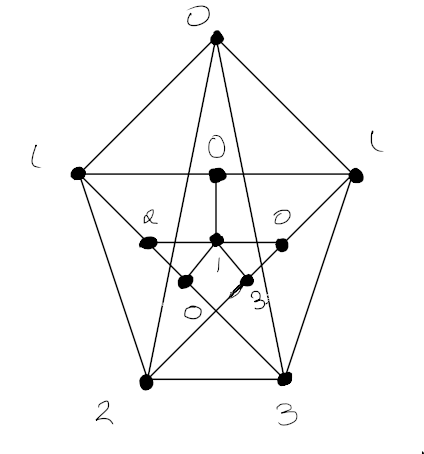
\includegraphics[scale=0.3]{Grafo10}
\end{center}

Ahora considere el siguiente subgrafo de $G$:

\begin{center}
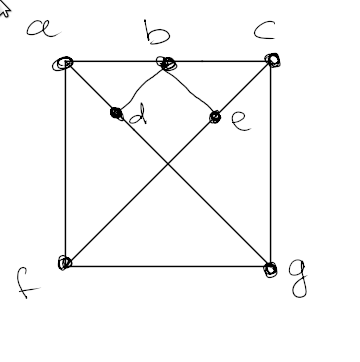
\includegraphics[scale=0.3]{Subgrafo10}
\end{center}

(Aquí los números denotan nombres de las aristas y no colores, como en el caso
anterior). Pues contiene a $C_3$ necesitamos al menos tres colores para
colorearlo propiamente. Asuma que existe un coloreo propio de tres colores. Los
dos $C_3$s se colorearán con los colores necesarios; por ejemplo, $c(a) = c(c) =
0, c(b) = 1, c(d) = c(e) = 2$. El único color disponible para $f$ es $1$; y si
se colorea a $f$ con $1$ no existe ningún color disponible para $g$ (y
viceversa). Es decir, no existe un coloreo propio de tres colores. 

El resultado anterior implica que $\chi(G) \geq 4$. Pero ya dimos un coloreo
propio de cuatro colores de $G$. Luego $\chi(G) = 4$.


\pagebreak 

\begin{problem}
    Igual que el anterior pero con un $C_7$.
\end{problem}

Es fácil notar que Greedy da un coloreo propio de $4$ colores, con lo cual
$\chi(G) \leq 4$. Pues $C_7 \subseteq G$, $\chi(G) \geq 3$. Es decir, $\chi(G)
\in \left\{ 3, 4 \right\} $. Es fácil encontrar un subgrafo de $G$ que no puede
colorearse propiamente con $3$ colores, lo cual concluye la prueba.

\pagebreak 

\begin{problem}
    Sea $G = (V, E) $ un grafo tal que $\chi(H) < \chi(G)$ para todo $H
    \subseteq G$. Probar que $\chi(G) \leq \delta + 1$.
\end{problem}

Asuma que $\chi(G) > \delta + 1$. Esto implica que $\delta < \chi(G) - 1$. Sea
$G'$ el grafo inducido por un vértice de grado $\delta$ y todos sus vecinos. Es
trivial observar que en el peor caso este grafo tiene $\chi(G') = \delta + 1$,
Pues $G$ es crítico, tendríamos que $\delta + 1 < \chi(G)$, lo cual contradice
la hipótesis.

Pues existe al menos un caso que contradice la hipótesis, y la hipótesis es
general, la contradicción es general. Es decir, $\chi(G) \leq \delta + 1$.








\end{document}



